\documentclass[12pt]{article}
\usepackage[utf8]{inputenc}
\usepackage{xcolor}
\usepackage{graphicx}
\usepackage{listings}
\usepackage{epstopdf}
\usepackage{etoc}
\usepackage{pdfpages}
\usepackage[capposition=top]{floatrow}
\usepackage{pdflscape} % landsacpe package
% set font to times
%\usepackage{mathptmx} % times!!! 
%\usepackage[T1]{fontenc}
\usepackage{amsmath}
\usepackage{soul}
\usepackage[left=2.5cm, right=2.5cm, top=2.5cm, bottom =2.5cm]{geometry}
\usepackage{natbib}
%\usepackage[natbibapa]{apacite}
%\usepackage{apacite}
%\bibliographystyle{apacite}
\bibliographystyle{apa}
%\renewcommand{\footnotesize}{\fontsize{10pt}{11pt}\selectfont}
\usepackage[onehalfspacing]{setspace}
\usepackage{listings}
\renewcommand{\figurename}{\textbf{Figure}}
\renewcommand{\hat}{\widehat}
\usepackage[bf]{caption}
\usepackage{tikz}
%\begin{comment}
%\usepackage[headsepline,footsepline]{scrlayer-scrpage} % has to come before package!!! otherwise option clash
%\usepackage{scrlayer-scrpage}
%\pagestyle{scrheadings} % kopfzeile/ fußzeile
%\clearpairofpagestyles
%\ohead{}
%\ihead{\textit{Redistribution, Demand and  Sustainable Production}}
%\cfoot{\thepage}
%\pagestyle{plain} % comment this one to have header
%\end{comment}
\usepackage{comment}
 \usepackage{siunitx}
  \usepackage{textcomp}
\definecolor{sonja}{cmyk}{0.9,0,0.3,0}
%\definecolor{purple}{model}{color-spec}
\usepackage{amssymb}
\newcommand{\ar}{$\Rightarrow$ \ }
\newcommand{\frp}[2]{\frac{\partial{#1}}{\partial{#2}}}
\newcommand{\tr}[1]{\textcolor{red}{#1}}
\newcommand{\vlt}[1]{\textcolor{violet}{#1}}
\newcommand{\bl}[1]{\textcolor{blue}{#1}}
\newcommand{\sn}[1]{\textcolor{sonja}{#1}}
%%% TIKZS
\usepackage{tikz}
\usepackage{times}
\usetikzlibrary{mindmap,trees}
\usetikzlibrary{backgrounds}
\usetikzlibrary{tikzmark}
\usetikzlibrary{decorations.markings}
\usepackage{tikz-cd}
\usetikzlibrary{arrows,calc,fit}
\tikzset{mainbox/.style={draw=sonja, text=black, fill=white, ellipse, rounded corners, thick, node distance=5em, text width=8em, text centered, minimum height=3.5em}}
\tikzset{mainboxbig/.style={draw=sonja, text=black, fill=white, ellipse, rounded corners, thick, node distance=5em, text width=13em, text centered, minimum height=3.5em}}
\tikzset{dummybox/.style={draw=none, text=black , rectangle, rounded corners, thick, node distance=4em, text width=20em, text centered, minimum height=3.5em}}
\tikzset{box/.style={draw , rectangle, rounded corners, thick, node distance=7em, text width=8em, text centered, minimum height=3.5em}}
\tikzset{container/.style={draw, rectangle, dashed, inner sep=2em}}
\tikzset{line/.style={draw, very thick, -latex'}}
\tikzset{    pil/.style={
		->,
		thick,
		shorten <=2pt,
		shorten >=2pt,}}
\tikzstyle{every edge}=  [fill=orange]  
% other stuff
\newcommand{\innermid}{\nonscript\;\delimsize\vert\nonscript\;}
\newcommand{\activatebar}{%
	\begingroup\lccode`\~=`\|
	\lowercase{\endgroup\let~}\innermid 
	\mathcode`|=\string"8000
}
%\usepackage{biblatex}
%\addbibresource{bib_mt.bib}
\usepackage{ulem}
\title{Growth, the Environment, and Inequality\\ \small{the political economy of environmental policies}}
\date{Sonja Dobkowitz\\ Bonn Graduate School of Economics\\ %University of Bonn\\
\vspace{1mm}
%Preliminary and incomplete\\
First version: November 27, 2021\\
This version: \today }
\usepackage{graphicx,caption}
\usepackage{hyperref}
\usepackage{minitoc}
\setcounter{secttocdepth}{5}
\usetikzlibrary{shapes.geometric}

% for tabular

%\usepackage{array}
\usepackage{makecell}
\usepackage{multirow}
\usepackage{bigdelim}

\renewenvironment{abstract}
{\small
	\list{}{
		\setlength{\leftmargin}{0.025\textwidth}%
		\setlength{\rightmargin}{\leftmargin}%
	}%
	\item\relax}
{\endlist}
\begin{document}
%	\includepdf[pages=-]{../titlepage.pdf}
	\maketitle
	
\section{Motivation}

\paragraph{Costs to sustainable production \ar reduction in growth necessary?}
\tr{a gradual approach and not categorised}
Due to climate change and vital threats to biodiversity we need to reduce the consumption of resources. % why this?/ Resource consumption= to emissions??? 
Macroeconomic research has largely focused on a green \textit{recomposition} of consumption. However, doubt has been raised if a recomposition of production alone suffices to fight climate change. 
Arguments which question the pure recomposition approach are, for instance, the use of nature as a sink \citep{Dasgupta2021}, failure of a decoupling of production and resource usage despite a  shift to sustainable technologies in recent years (\textit{degrowth book}), rebound effects of demand, or the existence of limiting factors  and the regenerative capacity of the planet.\footnote{\ For more arguments see article on simplicity movement.\\ Also: agricultural sector as an example}
Given the uncertainty about the possibilities of sustainable technologies to decouple resources and production, this paper draws attention to a world, in which a recomposition of production is not enough to comply with  planetary boundaries. 
The novelty is the introduction of an upper bound on the reduction of resource usage in the sustainable sector (\textit{hence there is some resource needed in the sustainable sector!}) in a macroeconomic analysis of environmental policies. %(\textit{Parameter values such that with the upper bound on technology today's consumption levels (of the rich) cannot be met.} SEEMS TOO RESTRICTIVE) 
As a result, consumption growth will eventually have to cease (or become negative) in order to respect planetary boundaries. %(\textit{postgrowth! not degrowth with this motivation }) 
%How much time remains for consumption growth to stop? One could argue not much due to uncertainty, irreversibility.

\paragraph{Research Question (What)}
 What is the optimal policy in such a scenario, a scenario where sustainable technology also exerts some negative externality on the environment.
 % (tipping point) is already very high (assumption of where we are relative to tipping point)? \ar make the distance from the tipping point a parameter on which results should depend.

\paragraph{How}
In the first part of the paper, I study this question in a representative agent world under a Ramsey planner. 
It is unclear a-priori if a reduction in output is indeed  a feature of the optimal policy. A trade-off not only arises under the assumption of non-satiated preferences, but also once a directed technical change is taken into account. 
On the one hand, a reduction in output in general reduces resource consumption and waste directly. On the other hand, innovations are triggered by a market size effect (cite Acemoglu). As the market size and hence expected profits of innovation reduce, technological progress in general and in the clean sector in particular might diminish. 
Evaluating the results, I give special attention on the effect on consumption and labour growth. Is it the case that as advocated by proponents of a reduction approach that consumption falls under the optimal environmental policy? 




Given that a reduction policy is associated with costs on the household side, it is important to extend the analysis of a reduction policy into a political economy setting. This constitutes the second part of the paper. 
First, the optimal policy resulting from the Ramsey problem under the assumption of a representative agent is evaluated in a model which features household heterogeneity. This approach allows to clearly see the consequences of the optimal policy resulting in the first part on (1) inequality, and (2) interactions of  inequality and the environmental externality. 

Some stylized facts on inequality environmental production are build into this extended model to assess  the effects of the optimal policy. First, the share of high and low-skilled workers varies across the clean and dirty sector. \cite{Bowen2018CharacterisingComposition, Consoli2016DoCapital} provide evidence for the share of high-skilled labour being higher in the clean sector. A reduction in labour supply by the rich (which might be more elastic to a reduction in labour income), could therefore increase costs of production in this sector by more than it does in the dirty sector. Which again could rise the price of sustainable produce, thereby, ceteris paribus, reducing the budget share of the clean good in households consumption baskets. In contrast, a price effect positively directs innovation towards the clean sector. 
\footnote{\ Could add heterogeneity in firm ownership and investment. }

\textbf{Effects on inequality}

I will then compare the optimal policy in the representative agent economy, to the optimal policy with inequality. This exercise sheds light on the role of inequality on the optimal environmental policy. 

In the third part, I will study the policy chosen by a \textit{democratically} elected government. 


\paragraph{Model}
The key contribution of the paper is to add environmental costs to ``clean'' production which  will ultimately imply a limit to consumption growth.
  (\textit{check consumption evolves in the AA model under the optimal policy})  
  endogenous directed technolgical innovation following  \cite{Acemoglu2012TheChange} into the model. Furthermore, in an extension, I allow for income-dependent marginal propensities to consume so that aggregate demand for green products varies with the distribution of income. When income of the poor falls in reaction to a drop in consumption by the rich, for instance, they might revert to consume a higher share of an unsustainable yet cheaper good. This again mitigates the reduction in resource consumption. 


 
\paragraph{Working time reduction\ar endogenous labour supply}
A policy that has been advocated for by  proponents of a reduction policy is a decline in working time. A reduction in working time, the argument runs, diminishes income, which again reduces today's consumption due to a lower budget.
(\cite{Schor2005SustainableReduction} does not really suggest a mechanism)
In addition, with non-separable preferences, a reduction in labour diminishes the marginal utility of consumption thereby indirectly reducing demand. 

In addition, a reduction in consumption might even not have a devastating effect on utility under the assumption of social preferences or some sort of addiction (UTLITY SPECIFICATIONS WITH HABITS DO NOT FEATURE ZERO GROWTH?)


A common assumption in the literature on working time reduction are endogenous preferences, which may positively rely on past consumption or some measure of societal consumption. Reducing income, then, also reduces 


Therefore, in the model presented here, labour supply is elastic. Households choose how much labour to supply. DO I NEED TO INTRODUCE FRICTIONS IN THE LABOUR MARKET HERE? such as: fixed costs per worker employed, unemployment benefits? 



\section{Plan for the paper: The quantitative experiment}
\begin{enumerate}
\item Calculate the optimal policy in a representative agent model (should be the same as for some politician?)\ar gives the optimal environmental policy absent inequality\\
\ar trade-off: reduction might have a negative effect on recomposition


\item A reduction in consumption growth/ employment is politically delicate \ar look at political economy of such a policy. \\
1) What effects does the policy resulting in bullet point above have on inequality?
2) What would a political government choose given inequality? 
\ar study the effects of a reduction on inequality

\item Plug in optimal environmental policy in a model with inequality (two households) 
\item Here analyse: how does inequality change the effect of the optimal environmental policy on the externality?; What are the consequences for different income groups?
\item In full model: Ramsey planner and Politicians (democratic politician bases policy on opinion) 
\end{enumerate}
\section{Fields connected by the project}


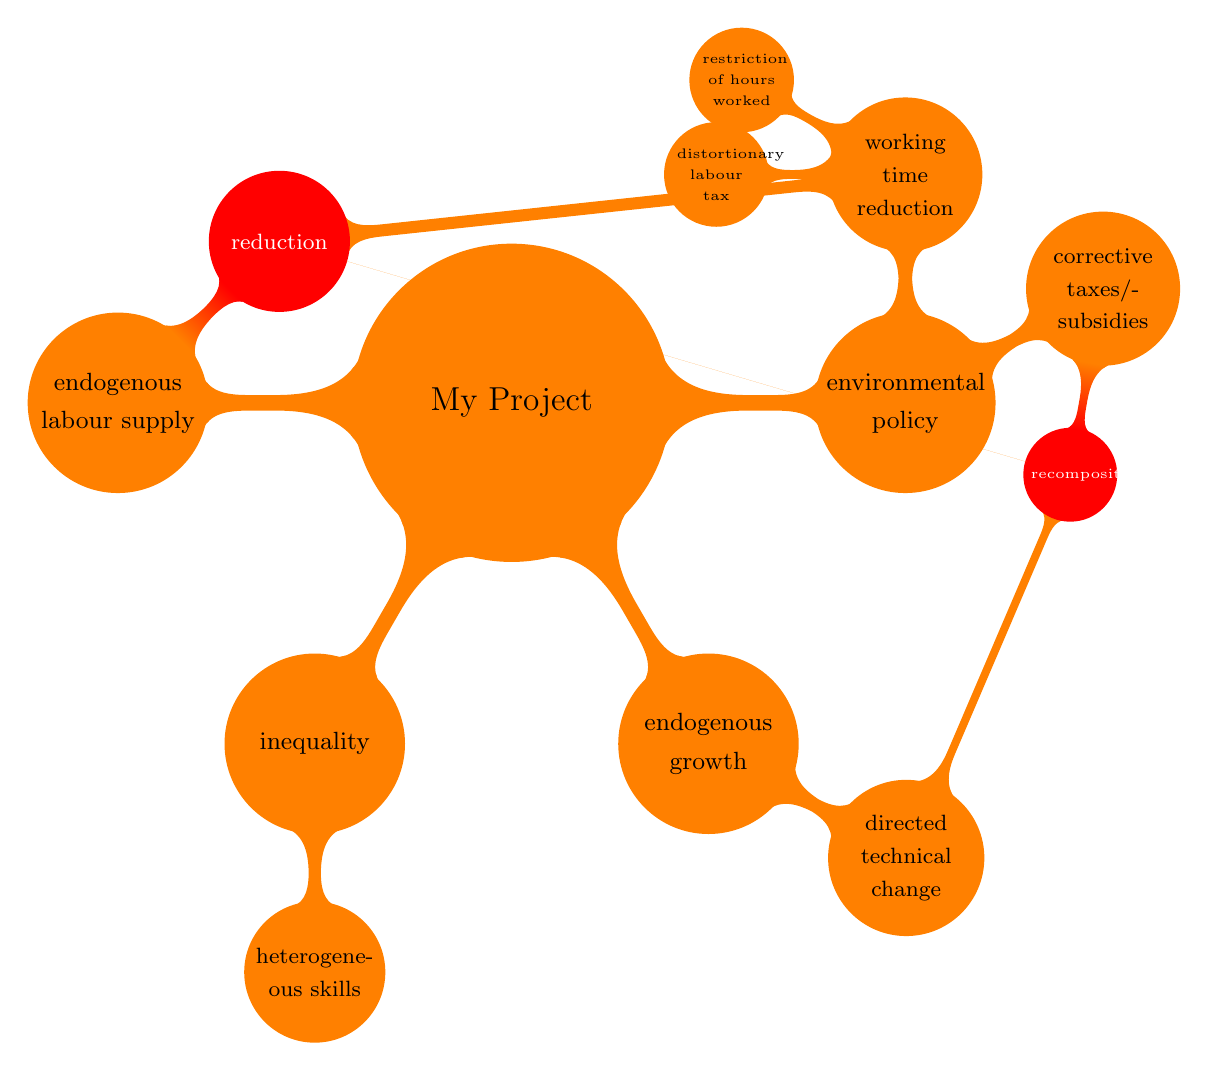
\begin{tikzpicture}[]
\path[mindmap,concept color=orange,text=black]
node[concept] {My Project}
[clockwise from=0]
child[] {
	node[concept] {environmental policy}
	[clockwise from=90]
	child { node[concept] (wtr)  {working time reduction} [clockwise from=180]
		child {node[concept] {distortionary labour tax}}
		child {node[concept] {restriction of hours worked}}
			}
	child { node[concept] (mainstream) {corrective taxes/subsidies}
	[clockwise from=-100]
	child [ concept color=red, text=white] { node[concept] (recomposition) {recomposition} }
	 }
}  
child[concept color=orange] {
	node[concept] (endg) {endogenous growth}
	[clockwise from=-30]
	child { node[concept] (dtc) {directed technical change} }
}
child[concept color=orange] { node[concept] {inequality} 
[clockwise from=-90]
child { node[concept] (hetskill) {heterogene-  ous skills}} 
}
child[concept color=orange] { node[concept] (endlab) {endogenous labour supply} [clockwise from=45]
child [ concept color=red, text=white] { node[concept] (reduc) {reduction}} 
};

\begin{pgfonlayer}{background}
\draw [circle connection bar ]
(recomposition) edge (dtc)[color=orange]
(reduc) edge (wtr) [color=orange];
\end{pgfonlayer}


\draw[->,  black] (reduc) edge (recomposition);

\end{tikzpicture}


\section{Literature}
\subsection{Endogenous growth/ directed technical change}
\begin{itemize}
	\item \cite{Acemoglu2012TheChange}
	\begin{itemize}
		\item focus on climate change \ar how would model change if focusing on nature as a whole (loss of biodiversity, acid oceans etc...)
\item 	Disaster and risk of non-existence \ar There is a disaster in their paper, and a point of no return. However, pollution does not reduce productivity; and there is no limit to the sustainable sector (no costs in terms of resource use, no waste); further, sustainable sector does not at all rely on nature as an input
\item no reversibility problem before point of no return (which might be the case with eg biodiversity)
	\end{itemize}	
	\item \cite{Eriksson2018PhasingChange}
	\begin{itemize}
\item directed technical change with  a low elasticity of substitution between dirty and clean goods \ar How motivated?
\item perpetual subsidy and increasing tax on the polluting good; pollution tax payments are a constant share of income; modest growth drag
\item no endogenous labour supply nor non-clean technology!
\item Eriksson's model even allows to phase out the polluting part of the dirty good. 
	\end{itemize}
\item \cite{Acemoglu2016TransitionTechnology}
\begin{itemize}
\item different modeling of competition between clean and dirty inputs
\item stressing this model to be a micro model...
\item in contrast to \cite{Acemoglu2012TheChange} final good producers choose which technology to use \ar firms are not sector specific but they use what maximises profits 
\item[\ar] In reality could think of a differentiation between profit-maximising firms and socially responsible firms which are committed to using the cleanest technologys
\end{itemize}
\item \cite{Acemoglu2002DirectedChange}
\begin{itemize}
\item 2 different labour inputs to two sectors
\item there are costs associated with research which is not the case in \cite{Acemoglu2012TheChange}; this is the \textit{lab equipment model} which uses the final good as input to innovation!  (spending!); the alternative \textit{knowledge-based R\&D} specification: need knowledge spillovers from the past to sustain growth; ``standing on the shoulders of giants"
\item \textit{knowledge based R\&D}: 
\begin{itemize}
\item scientists carry out research, there is a constant supply of scientists $=S$
\item with only one sector growth would be proportional to S
\item can allow knowledge spillover from both sectors and not only the given one... \\
$\Delta N_l=\eta_L N_l^{(1+\delta)/2}N_z ^{(1-\delta)/2}s_L$; $s_L$ scientists allocated to sector $L$; $\eta_L$: costs of innovation in sector L
\item this formulation generates \textit{state dependence} if $\delta \neq 0$.                                                                                                                                                                                                                                                                                                                                                                                                                                                                                                                                                                                                                                                                                                                                                                                                                                                                                                                                                                                                                                                                                                                                                                                                                                                                                                                                                                                                                                                                                                                                                                                                                                                                                                                                                                                                                                                                                                                                                                                                                                                                                                                                                                                                                                                                                                                                                                                                                                                                                                                                                                                                                                                         
\end{itemize} 
\item machine producers and innovations are the same unit
\item innovation is on the variety of machines! \ar there are new machines being invented not the technology of existing firms
\end{itemize}
\end{itemize} 

\subsection{Limits to endogenous growth}
\begin{itemize}
\item \cite{Stokey1998AreGrowth}
\item \cite{Jones2016LifeGrowth} VERY NICE WRITING STYLE AND PRESENTATION OF RESULT! (caveats and how to interpret results)
\begin{itemize}
\item technologies increase or decrease risk of staying alive (health, nuclear, pollution) \ar Roussian Roulette
\item Do research and consumption growth continue forever in such a setting? 
\item answer depends crucially on preferences; but, in conventional specifications, including log utility, \textbf{the value of life rises faster than consumption}
\item[\ar] consumption growth below what is feasible! 
\item how does he include risk? \ar probability that research leads to death (seems like to rough a short cut to me in the context of environment: could have instances that decide on whether innovation is used; then again, the consequences may not be foreseen (e.g. fracking))
\item exponential growth possible if growth rate is higher than expected costs of disaster
\item limit to growth when IES above 1; sufficiently rich generations decide against further growth when risk of losing life is too high
\item transition: reallocation of scientists away from consumption sector towards life-saving sector. 
\end{itemize}
\item \cite{Brock2005ChapterEmpirics}
\begin{itemize}
\item they argue that there is no non-pollution free technology! (p.1760 f.)
\item therefore, there cannot be growth in incomes when environmental boundaries are to be respected
\item from p. 3
\begin{quote}\textit{
Nature’s other role – its role as a sink for unwanted by-products of economic activity – has typically been given less attention. As a sink, nature dissipates harmful air,
water and solid pollutants, is the final resting place for millions of tons of garbage, and
is the unfortunate repository for many toxic chemicals. When the environment’s ability
to dissipate or absorb wastes is exceeded, environmental quality falls and the policy
response to this reduction in quality may in turn limit growth. Growth may be limited
because reductions in environmental quality call forth more intensive clean up or abatement efforts that lower the return to investment, or more apocalyptically, growth may
be limited when humans do such damage to the ecosystem that it deteriorates beyond
repair and settles on a new lower, less productive steady state.}
\end{quote}
\item no optimal policy analysis

\end{itemize}
\end{itemize}


\subsection{Working-time reduction}
\begin{itemize}
\item \cite{Schor2005SustainableReduction}
\begin{itemize}
\item discusses evolution in working hours in developed economies
\item argues against ``neoclassical'' logic that consumption growth implies a reduction in labour supply (preferences determine market); instead, she advocates endogenous preferences which imply that as income rises there is no desire to lower working time 
\item[\ar] policies should stem (eindämmen) income increases instead of reducing current consumption! (this is what is harmful, not future income reduction). This theory relates to \textit{loss aversion} (Kahnemann and Tversky 1984,) of what I have instead of future profits...\textit{status quo bias} (Samuelson and Zeckhauser, 1988), \textit{endowment effects} (Thaler, 1980)
\item endogenous preferences: desires change so that I like what I have once I have it; This is different from social preferences and habits yet, these are also endogenous  
\item she does not give a structured explanation of how a working time reduction should affect environmental externalities; she drops some vague ideas: 1) negative effect if leisure activities are environmentally costly such as traveling...; 2) due to more time a reduction in the consumption of speed and convenience which are ecologically costly;
\item presents some ideas on how hours reduction should be done: per worker, per job, egalitarian or not... (she suggests egalitarian arguaing that an unequal reduction implies opposition of those who work high hours)
\item she suggests there might be a trade-off in growth: a) increasing sustainable technology $\uparrow$ environment, b) increasing incomes \ar consumption $\downarrow$ environment
\end{itemize}

\item \cite{Pullinger2014WorkingDesign}
\begin{itemize}
\item how to implement a working time reduction so that it also increases happiness?
\item less work\ar less consumption (therefore especially under the rich)
\item happiness to be derived from more free time
\item he looks at voluntary working time reduction possibilities in the Netherlands and Belgium
\item working time reduction over the life cycle
\item \textbf{mechanism:} productivity growth to be translated into leisure growth and not consumption growth
\item drop in wellbeing if utility based on absolute consumption; 
\item rise in wellbeing possible through a reduction in the disutility from labour (e.g. stress, )
\item here: \textbf{voluntary working time reduction}
\item Netherlands/Belgium: ``Life course approach'' \ar a right to flexibly reduce working time
\item[\ar] discusses policies to support preferences for voluntary WTR
\item more conventional measures to reduce working time: 
maximum working hours, use-specific WTR (childcare); 
\end{itemize}
\item What are the macroeffects on a working time reduction? Hypothesis: higher wage in the reducing sector \ar inequality, externality
\item paper by \cite{Cieplinski2021EnvironmentalReductionb} more macro approach \ar explore trade-offs of WRT on externality
\begin{itemize}
\item macro approach to the effect of working time reductions
\item unclear mechanisms, \textit{``interaction of WTR and GDP ''}...?
\item 
\end{itemize}
\item \cite{Alvarez-Cuadrado2007EnvyHours}
\begin{itemize}
\item in a model with envy he shows that a restriction on working hours comes close to the optimal allocation implemented through a subsidy on leisure or general consumption tax.
IDEA \ar Sonja: couldn't it even be better to have working time restrictions in a model with inequality as the overall consumption tax should hurt them more (regressive) On the other hand, a subsidy on leisure could also be more appreciated by the rich, as it hurts them less to reduce consumption. Restrictions on hours worked could then not hurt the poor...?
\item in the model, hh derive utility from a weighted consumption bundle of absolute and relative consumption! The weight on relative consumption determines envy.
\item endogenous labour supply
\item the utility function is not separable in consumption and leisure \ar more leisure \ar higher MU of consumption \ar THIS might be relevant for the mechanism on how a working time restriction impacts demand! Other than an initial change in income which might be done away by a rise in wages?
\item taxes on capital and labour income and on consumption
\item inefficiently high levels of consumption and labour supply as hh overvalue consumption due to envy; or better, as they do not incorporate the negative utility effect on other households through their consumption plus on themselves. 
\item[\ar] \tr{with a negative externality of consumption (in general, all consumption) on the environment, the effect should be similar. Should be optimal to lower total consumption not only through corrective tax. }
\item envy implies to margins of the externality: on the intertemporal trade-off (for non time-separable, iso-elastic preferences) and on the static trade-off between leisure and consumption
\item optimal tax rates, efficient allocation restored: $\frac{1-\tau_w}{1+\tau_c}=1-\gamma$ a rise in $\tau_w$ tax on labour income, or a rise in tax on consumption, starting from the laissez-faire. 
\item if optimal policy is not available: restriction on hours worked
\item empirics on reductions in hours worked
\item \tr{socially more preferred policy to lower working hours (mandatory holidays, workweek limitations) as opposed to higher labour income taxes or consumption taxes}
\item implementation working time reduction: upper bound on labour is the efficient level! 
\item he studies transitions from the laissez-faire to the new ss once the efficient level of hours worked is introduced; the transition is different across optimal and worktime reduction policy
\item transition:
\begin{enumerate}
\item imply upper bound on labour supply
\item agents choose highest feasible working time level
\item at the fixed capital stock, drop in labour implies drop in output and consumption (supply side effect!)
\item decrease in consumption and capital 
\end{enumerate}
\item expects higher welfare losses when agents are heterogeneous
\item what if leisure and consumption where separable in utility... no adjustment in consumption when wages adjust?
\item effects of sudden drop in labour supply: 1) reduced income \ar reduced consumption; 2) with non-separable preferences, also a higher/lower MU of consumption as leisure rises;
lower labour supply \ar higher MPL at fixed capital stock, \ar higher wage rate \ar higher income at constant labour \ar higher consumption;
higher demand \ar Keine Ahnung;
capital stock decreases as MPK reduces with lower labour supply \ar lower savings rate\ar higher demand today... 
\end{itemize}
\end{itemize}

\subsection{Skill and environment}
\begin{itemize}
\item \cite{Borissov2019CarbonDevelopment}
\begin{itemize}
\item skills are crucial a determinant of green growth as the labour required for green production is special: higher skills/ higher human capital accumulation
\item their focus seems not to lie on inequality!
\item their idea: requiring non-developed countries to reduce emissions \ar higher carbon taxes \ar increase in human capital investment since the green sector uses high-skilled labour \ar economic growth! (\textit{how measured?}) \ar a win-win situation
\item North-South knowledge spillover: if the carbon tax leads to knowledge growth in the green sector this might spread to the South even if the South itself does not levy a pollution tax
\item human capital accumulation is the driver of growth in this model (not innovations! no directed technical change)
\item no a-priori inequality in their model! Skill is a choice variable! 
\end{itemize}
\end{itemize}

\section{Arguments Recomposition versus Reduction}
\subsection{Arguments against the sufficiency of sustainable technological growth/ recomposition}
Most compellent argument against unlimited growth: sustainable sector also consumes nature; waste through 
\begin{itemize}
\item missing decoupling: rise in resource usage despite more clean technology \citep{Alexander2012TheContext}
\item rebound effects (look at Taylor and Tilford, 2000, as cited in \cite{Schor2005SustainableReduction}); XXX Paradox \citep{Alexander2012TheContext}
\item moral obligation against less developed countries and those consuming at a lower bound of consumption \citep{Alexander2012TheContext}
\item slow diffusion of green technologies \citep{Schor2005SustainableReduction}; Does she give evidence?
\item why price reductions are not a good indicator of scarcity: no property rights \citep{Schor2005SustainableReduction}
\item \cite{Cohen2019AnnualSubstitutable}: Is natural capital really substitutable?
\begin{itemize}
\item Sonja: only relying on clean sector as in AA means nature is fully substitutable in production by capital and labour
\item find low to moderate substitutability eg in agricultural land use, or industrial energy use
\end{itemize}
\item \cite{Arrow2004AreMuch}
\begin{itemize}
\item following \cite{Cohen2019AnnualSubstitutable} they show/ argue that economic development was already impeded by natural degradation in 2004
\end{itemize}
\end{itemize}



\subsection{Arguments for unlimited sustainable growth}
\begin{itemize}
\item \cite{EndGrowthAghion1998} in Chapter 5 are supposed to show that there might be no end to growth ``\textit{when environmentally-friendly innovations are allowed.}'' (S.134 \cite{Acemoglu2012TheChange})
\item notes from \cite{EndGrowthAghion1998} Intro to Chapter 5
\begin{itemize}
\item ``\textit{Whether or not [under which conditions] growth can be sustained is the central question to which endogenous growth theory is addressed.}'' (p.151)
\item  Conclusions: ``\textit{chances of achieving sustainable growth depend critically on maintaining a steady state flow of technological innovations}''
\item ``\textit{If it had not been for resource-saving innovations it is unlikely that \textit{our finite planet} could have supported the expansion in material welfare that as taken place since the industrial revolution.}'' \ar There is progress in technology, i.e., a push towards a better translation of resources into output
\item ``\textit{Although there is nothing in endogenous growth theory implying that these trends will necessarily sustain development into the indefinite future, nevertheless the theory does imply that with enough innovations [ain't that the question whether this exists], and the right direction of innovations, such an outcome is at least within the realm of possibility.}''
\\
The question for possibility remains unsolved since it is unclear whether \textit{enough innovations} are possible!  \textit{enough} can be understood as that it is possible. Hence, assuming what has to be shown... 
\item "\textit{It turns out to be crucial for sustainability [...] that the technology for \textbf{producing knowledge} is generally \textbf{cleaner} than that for \textbf{producing physical capital}}" \ar since the former is the source of sustainability
\item \textbf{Results}: 
\begin{itemize}
\item elasticity of intertemporal substitution in consumption must be lass than unity \ar do not respond too elastically to changes in the real rate; otherwise environmental quality below threshold level might become an option
\item finiteness of nonrenewable resources is less a problem for sustainable growth than the problem of environmental pollution (That is: nature as a sink!)
\item growth in the Schumpeterian model can be sustainable while taking natural constraints into account
\end{itemize} 
\end{itemize}
\item Optimal Growth in the AK and Schumpeterian Frameworks \citep[Chapter 5,][]{EndGrowthAghion1998}
\begin{itemize}
\item AK model: knowledge is capital; Schumpeterian model: knowdledge is distinct from more tangible capital 
\item the production function in \cite{Acemoglu2012TheChange} is a Schumpeterian approach: $Y= L^{1-\alpha}\int_{0}^{1}B(i)x(i)^\alpha$
\item the production of intermediate good i is given by $x(i)=\frac{K(i)}{B(i)}$ \ar that is: the more productive a good (higher B) the more capital is needed to produce it!
\item Leading edge technology in sector i: $B_i^{max}=max(B(i))$
\item result: unlimited growth is sustainable, \textit{because the common rate of return to the two kinds of capital does not diminish as more and more capital is accumulated} \ar hh are willing to postpone consumption as the growth rate exceeds their time preference. 
\item[\ar] the only trade-off which exists here is the one between consumption today and tomorrow. There are no external costs to consumption and saving
\item How is research related to $B$ in this model?
\item \textbf{adding sustainability aspects}:
\begin{itemize}
\item utility depends on environmental quality $E$
\item \textbf{pollution} deteriorates environmental quality; pollution $P$ is a function of output Y (+) and the intensity of pollution z (+)
\item \textbf{non-renewable natural resource} $S$, depleted by the rate of resource extraction
\end{itemize}
\item[\ar] is growth sustainable = whether or not there exists an optimal growth path along which the net national product grows without bounds! (p.158)
\item in the Schumpeterian model growth can be sustainable if the rate at which knowledge is accumulated is higher than that of capital accumulation, than the marginal product of capital is kept high and hh are willing to save! Which is the definition of sustainaing growth!
This is an optimality analysis: Trade-off: when output rises, the intensity of pollution has to reduce \ar reduces the social marginal product of capital \ar time preferences could become such that hh do not want to save up anymore... 
Knowledge has to make up for the reduction in the intensity of pollution in order for hh to continue saving (p.158 bottom)
\item[\ar] this argument focuses on the willingness to save, not on planetary boundaries
\item[\ar] this approach looks at an average degree of pollution intensity, as if aggregating the two sectors, \textbf{Can this pollution intensity $z$ be driven towards zero?} How is it determined? 
\item trade-off in Stokey's AK model (p.159)
\begin{itemize}
\item on the one hand, cleaner production \ar less pollution
\item on the other hand, cleaner production \ar lower TFP
\item for sustainable unbounded growth need to have $z\rightarrow0$ in the long-run. \textbf{What if in the mean time, before $z\rightarrow0$ too much of the current output is produced,  so that pollution is too high despite the possibility of $z\rightarrow0$}? How to formulate this in the model? Is thi excluded as a possibility? How?
\item \tr{\textbf{Continue reading on p. 159`}}
\end{itemize}
\end{itemize}
\end{itemize}

\subsection{Scientific papers on planetary boundaries}

\subsection{Are there environmental costs to energy/ production modes considered ``clean''?}
\begin{itemize}
\item quora forum discussion on fossil versus nonfossil fuels (\url{https://www.quora.com/What-are-non-fossil-fuels}) \ar different definitions, nonfossil mainly renewable and if emission of CO2 can be made up for then also considered carbon-neutral (eg. burning a tree releases CO2 which the tree had absorbed before, then replanting a tree makes the whole thing carbon neutral.)
\item but there is also CO2 released
\item US authority on GHG \\ \url{https://www.epa.gov/ghgemissions/inventory-us-greenhouse-gas-emissions-and-sinks}
\end{itemize}
\section{Empirical Contribution}
Measure resource usage of clean products relative to non-clean sector...BETTER: provide evidence from already existing studies! Seems to be a boring exercise


\section{Model}
\subsection{Preferences}
In the baseline version of the model, there are standard preferences. Households care about the absolute amount of consumption and utility is monotonically increasing in consumption. 
In an extension: 
High consumption levels feature prominently in the literature suggesting a reduction of consumption for environmental reasons. In the economics literature, overconsumption has been shown to result from habits or social preferences. This paper places the environmental policy analysis in a model with habits/ social preferences as these seem to be the reason for high consumption levels, so that they should be taken into account in an analysis of potential reductions in consumption. 

\subsection{Inequality}

\noindent Income heterogeneity is introduced by
\begin{itemize}
\item skill heterogeneity
\item firm ownership
\item investment into research
\end{itemize}

\subsection{Pollution}
Build on \cite{Acemoglu2012TheChange} but make the sustainable sector also exert pollution but less (motivate by production of electric vehicles, solar panels, infrastructure for railways) or leading to waste.  
\subsection{Government}
\subsubsection{Objective function}
Political considerations and societal acceptance of environmental policies is a crucial aspect for environmental protection to succeed. 
In the second part of the paper, I, therefore, consider a government which searches to increases its chances on reelection. 
Three alternative ways to set up the government's objective function
\begin{enumerate}
	\item aggregation of utilities according to median voter?
	\item assuming the gov does not know utilities, it could search to maximise value measures such as employment rates, environment with weights that follow polls, opinions in society (use WVS data)\\ \ar How important is a change in electorate values towards environmental priority to prevent environmental disaster?\\
	Endogenise values relevant for votes \ar economic downturn \ar surge of prioritising economic growth, for instance
\end{enumerate}

\subsubsection{What policies can the government choose from?}
How is working time reduction in \cite{Schor2005SustainableReduction} implemented?
What structural biases does she see on the firm level? i.e., why do firms have an advantage to keep working hours per worker high?
\textit{Extension:} Model jobs posted as having a fixed number of hours.

Tax policies which might imply a reduction in consumption over time.

\subsection{The environment and planetary boundaries}

Read nature articles

\clearpage
\bibliography{../../../bib_2_0}
\addcontentsline{toc}{section}{References}
\end{document}